% -*- root: ../../../main.tex -*-
\subsection{Client Protocol}

Al fine di comprendere il funzionamento dell'algoritmo è necessario capire quali sono le modalità con cui i server interagiscono con i client.
RAFT è un algoritmo leader-based, di conseguenza è il leader che svolge i compiti principali, ed è anche l'entità che si occupa della comunicazione con i client.

	\subsubsection{Caso base}
	L'interazione di base tra il client e il leader del server, che va dalla sottomissione della richiesta alla ricezione del risultato di quest'utlima attraversa le seguenti fasi:

	\begin{enumerate}
		\item{\textbf{Sottomissione:}} il \textbf{client} sottopone la richiesta al leader.

		\item{\textbf{Presa in carico:}} il \textbf{leader} leader prende in carico la richiesta, accodandola al proprio log e replicandola sugli altri server.

		\item{\textbf{Commit:}} il \textbf{leader}, prima di poter procedere col soddisfare la richiesta, deve \textbf{assicurarsi} che venga fatto il \textbf{commit} della stessa, per avere la garanzia che sia stata replicata nella maggioranza dei log. 

		\item{\textbf{Esecuzione:}} assicuratosi che il commit sia avvenuto, e che quindi sia \textit{safe} computare il risultato, il \textbf{leader} fa eseguire l'istruzione alla propria \textbf{state machine}

		\item{\textbf{Risultato:}} ottenuto il risultato, il leader lo comunica al client.

	\end{enumerate}

	
	\subsubsection{Ricerca del leader}
	Per dare inizio alla scambio, il client deve \textbf{contattare il leader} del cluster. Nel caso in cui il client \textbf{non sappia} quale tra i server del cluster sia il leader è sufficiente che contatti \textbf{un membro qualsiasi} del cluster.
	Se un follower riceve una richiesta da un client, risponde con le \textbf{informazioni sul leader}, neccessarie affinchè il client possa \textbf{contattarlo direttamente}. 

	Questo meccanismo entra in funzione anche nel momento in cui, a seguito di un crash del leader, il client ha bisogno di scoprire l'identità di quello nuovo al fine di risottomettere una richiesta.  

	\subsubsection{Crash del leader}

	Abbiamo detto che nel caso in cui il client non riceva più notizie dal leader, ad esempio a causa di un crash di quest'ultimo, l'interazione si svolge nel seguente modo:

	\begin{enumerate}
		\item{\emph{Il \textbf{client} ritrasmette il comando ad \textbf{una qualsiasi} delle altre macchine. }}
		\item{\emph{Se la macchina contattata \textbf{non è il }\textbf{nuovo leader}, fornisce indicazioni su \textbf{a chi rivolgersi}.}}
		\item{\emph{Il \textbf{client} si rivolge al \textbf{nuovo leader} e, ad esso, \textbf{risottomette} la richiesta}}
	\end{enumerate}

	Questo iter \textbf{garantisce} che ogni richiesta verrà gestita, \textbf{prima o poi}, ma ancora \textbf{non è sufficiente} a garantire che venga eseguita \textbf{una e una sola volta}. 
	Può accadere che il crash del leader avvenga \textbf{dopo} l'esecuzione del comando, ma \textbf{prima} che sia comunicata la risposta al Client. 
	In questo caso il client non saprebbe che il comando è stato eseguito e ritrasmetterebbe la richiesta al nuovo leader il quale, nel momento in cui farà commit del comando, lo rieseguirà. In questo modo si avrebbe che il comando è stato eseguito \textbf{due volte}, il che non è accettabile.

	  \begin{figure}[H]
	    \centering
	    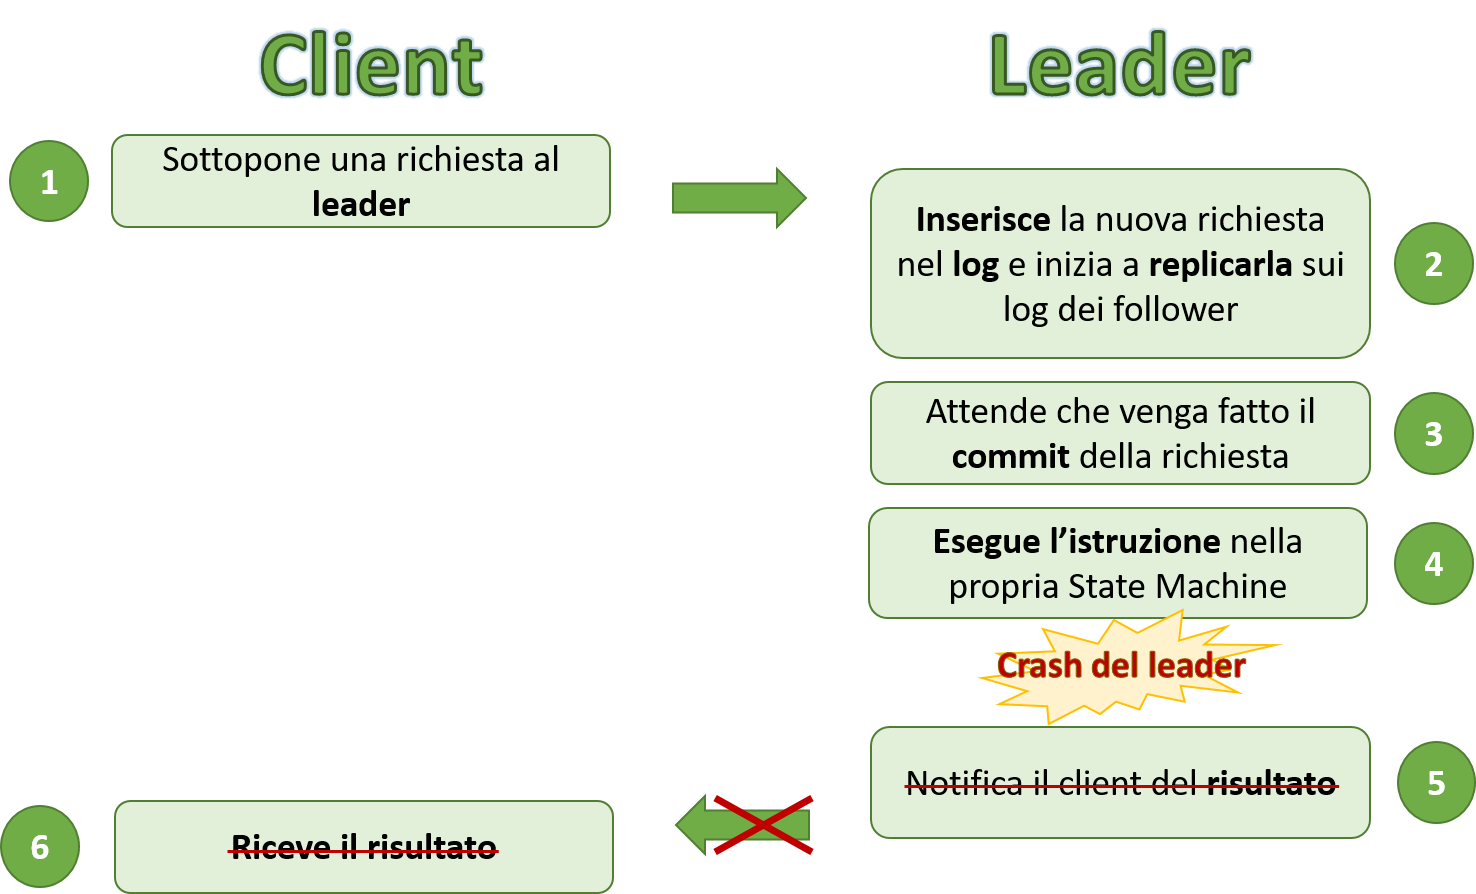
\includegraphics[width=0.90\columnwidth]{raft/clientProtocolSenzaID.png}
	    \caption{Lo schema mostra l'interazione di base tra il client e il leader. Nel caso in cui si verifichi un \textbf{crash del leader} nel punto evidenziato in figura, si corre il rischio che il client risottometta la richiesta al nuovo leader e che anche quest'ultimo la esegua, \textbf{violando} il vincolo secondo cui una richiesta debba essere eseguita esattamente \textbf{una e una sola} volta.  }
	    \label{fig:figure 12}
	  \end{figure}
 
 	\subsubsection{Introduzione di una exactly-once semantics}
 	Per garantire che uno stesso comando richiesto da un client non possa essere eseguito più di una volta, si introduce un \textbf{identificatore univoco} per ogni richiesta.  

 	\begin{itemize}
 		\item{{Il client genera di volta in volta l'identificativo e lo inserisce nella richiesta.}}
 		\item{{L'identificativo è contenuto nell'entry el log relativa alla richiesta}}
 		\item{{Se il leader riceve una richiesta con un identificativo \textbf{non presente} in una delle entry del proprio log si comporta come di consueto: 
 			\begin{enumerate}
 				\item{\emph{la accoda;}}
 				\item{\emph{inizia a replicarla;}}
 				\item{\emph{raggiunta la maggioranza dei consensi fa commit della stessa;}}
 				\item{\emph{la esegue}}
 				\item{\emph{comunica il risultato al client.}}
 			\end{enumerate}
 		}}
 		\item{Se il leader riceve una richiesta con un identificativo già \textbf{presente} in una delle entry del proprio log, si comporta in questo modo:
			\begin{enumerate}
 				\item{\emph{\textbf{non} la accoda;}}
 				\item{\emph{attende che ne venga fatto il commit (se non è già successo);}}
 				\item{\emph{la esegue (se non l'ha già fatto;)}}
 				\item{\emph{comunica il risultato al client.}}
 				
 			\end{enumerate}
 		}
 		
 	\end{itemize}

In questo modo si garantisce che un comando venga eseguito una e una sola volta: \textbf{exactly-once semantics}.

	  \begin{figure}[H]
	    \centering
	    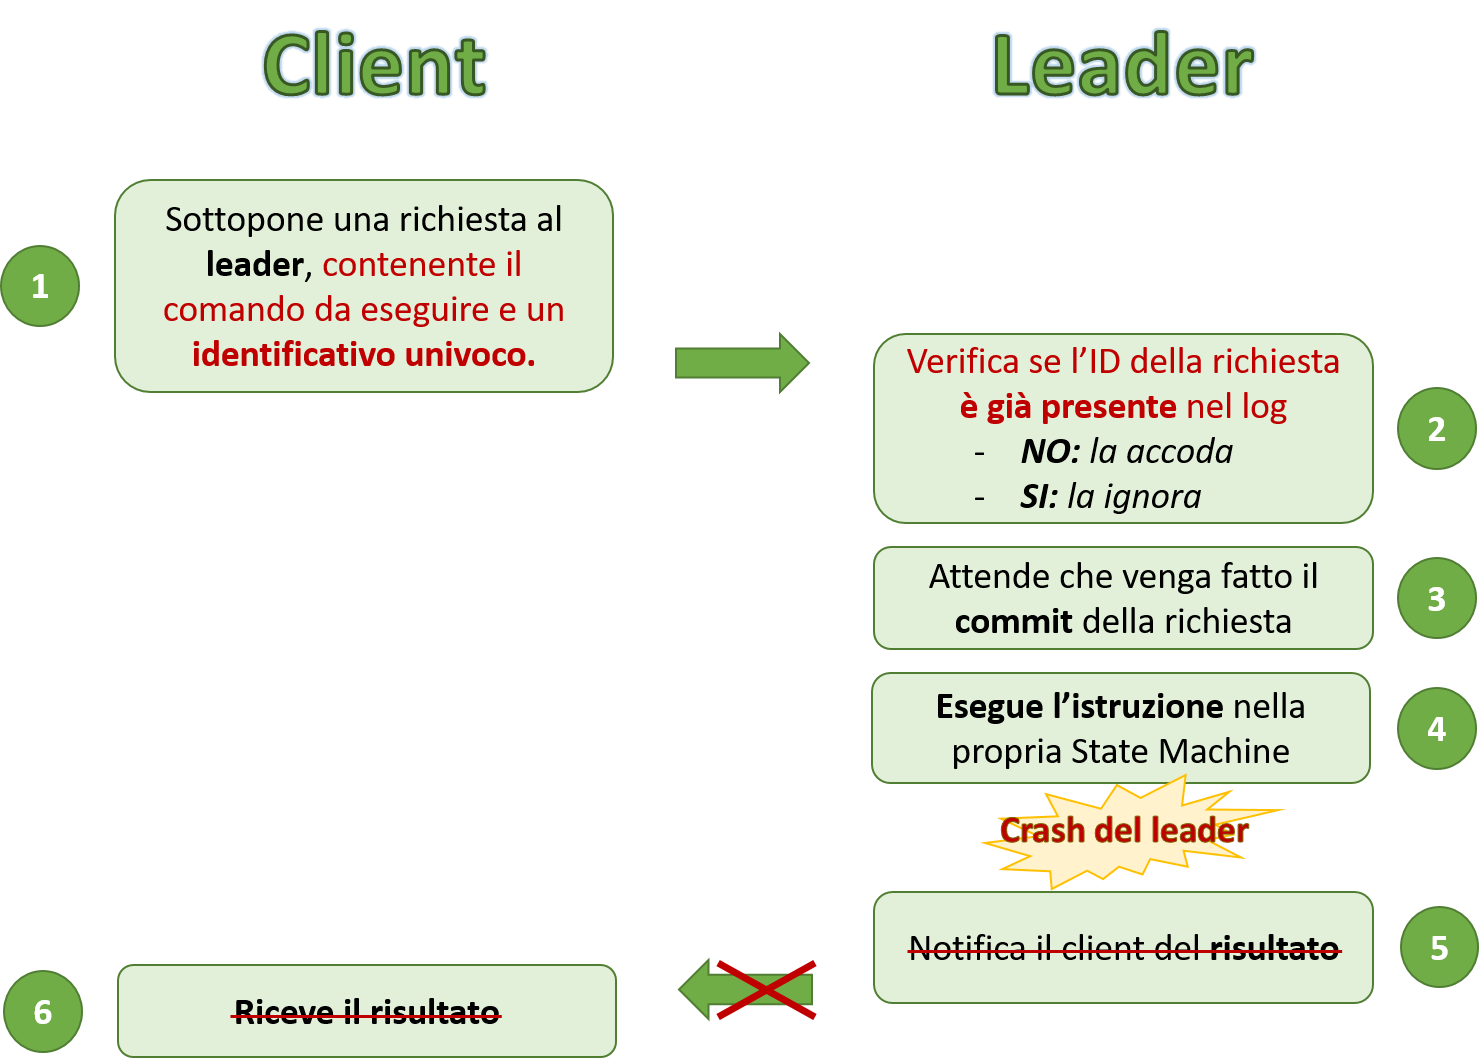
\includegraphics[width=0.90\columnwidth]{raft/clientProtocolConID.png}
	    \caption{\textbf{Interazione} tra client e leader che tiene conto dell'aggiunta di un \textbf{identificativo} per le richieste, al fine di \textbf{evitare} la \textbf{molteplice esecuzione} di una richiesta. Diversamente dal caso precedente, un crash del leader nel punto evidenziato \textbf{non porta alla violazione di alcuna proprietà}.}
	    \label{fig:figure 13}
	  \end{figure} 

	  \begin{figure}[H]
	    \centering
	    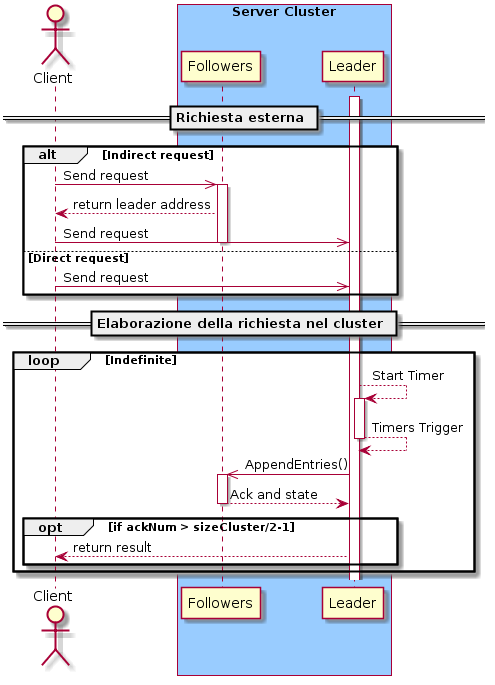
\includegraphics[width=0.90\columnwidth]{../plantuml/rendered/seqDiagrams/ClientRequest.png}
	    \caption{Rappresentazione completa dell'interazione tra il client e i server appartenenti al cluster.}
	    \label{fig:figure 14}
	  \end{figure} 
